\chapter{\IfLanguageName{dutch}{Inleiding tot Ansible en cloud-init}{Introduction}}
\label{ch:inleidingtotansibleencloudinit}

Dit hoofdstuk is een inleiding over cloud-init en Ansible. Eerst wordt Ansible besproken. Er wordt eerst wat algmene uitleg gegeven, daarna wordt iets dieper op ingegaan op de architectuur, playook, roles en de omgeving. Erna wordt er voor cloud-init hetzelfde gegaan. Eerst wordt er wat algemene uitleg gegeven. Daarna wordt er dieper ingegaan op de modules, Cloud config, omgevingen en systemen.


\section{Ansible}
Ansible is een open source IT configuration management en deployment tool. Ansible hun grote doel is om besturingssysteem configuratie en de implementatie van software te vergemakkelijken. Door dit allemaal onder 1 systeem te steken. De informatie werd gevonden met behulp van het document \textit{Ansible In Depth} \autocite{ansibleid}.

Ansible staat bekend als een systeem dat makkelijk te leren is als IT administrator, ontwikkelaar of manager. Het probeert er voor te zorgen dat het makkelijk te verstaan is en makkelijk om zelf op te bouwen. Zo kunnen nieuwe gebruikers dit eenvoudig en snel oppikken.Ze proberen uniek te zijn in toegankelijkheid voor gebruikers. Ze willen dat er veel aanpassingsmogelijkheid is voor de expertgebruikers. Maar ook zeer toegankelijk en eenvoudig voor nieuwe gebruikers.

\newpage
\subsection{Architectuur}
Eén van de belangrijkste verschillen tussen Ansible en andere configuratie management tools, is zijn architectuur. Ansible gaat uit van het ``push'' model. Ook is er geen additionele software nodig om machines bruikbaar te maken voor Ansible. Het heeft geen extra gebruikers of referenties nodig om te draaien. Het gebruikt gewoon de informatie die de user meegeeft. Daarbij hoort ook dat Ansible geen administrator of sudo toegang nodig heeft. Ansible wordt standaard bestuurt door een remote computer.

Dit zorgt ervoor dat Ansible veiliger wordt. Alleen de informatie die de gebruiker meegeeft wordt gebruikt. Een gebruiker die wel toegang heeft tot de server, maar niet tot de remote computer, kan geen aanpassingen pushen.

\subsection{Playbook - Roles}
Ansible voert de automatisatie en deployment uit via playbooks. Dit zijn yaml bestanden die beschrijven hoe de automatisatie moet verlopen. 

Deze playbooks bevatten verschillende ``plays'' die de automatisatie definiëren over verschillende hosts. Deze hosts staan bekend als de inventory. Elke ``play'' bevat verschillende taken die één, enkele of alle hosts moeten uitvoeren. Elke taak roept een Ansible module aan, een klein stukje code dat een specifieke taak uitvoert. Deze kunnen zeer simpel zijn, een bestand op een machine zetten of een specifieke package installeren. Maar ze kunnen ook complex zijn zoals een gehele CloudFormation opstarten in Amazon EC2. Figuur \ref{fig:playbook} is een voorbeeld van een playbook. 
\begin{figure}[!htb]
	\center{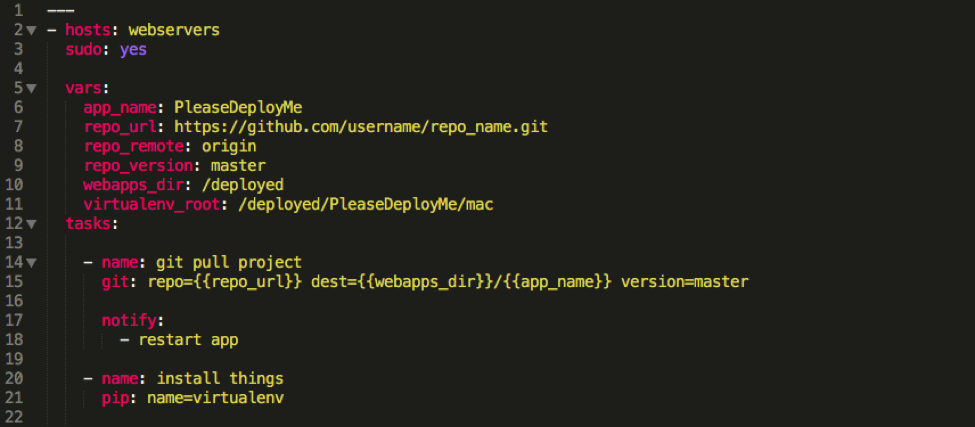
\includegraphics[width=0.9\textwidth]{img/playbookex.png}}
	\caption{Voorbeeld van een Ansible playbook. \autocite{ansibleplaybook}}
	\label{fig:playbook}
\end{figure}

Ansible is geschreven zodat als ze de playbook uitvoeren ook checken of deze task nog moet gedaan worden. Bijvoorbeeld als een Ansible taak is om een webserver op te starten, zal Ansible deze alleen uitvoeren als de webserver nog niet is opgestart. Dit staat bekend als idempotentie. Het zorgt ervoor dat de configuratie altijd snel en efficiënt wordt uitgevoerd.

\newpage
Met Ansible kunnen taken ook ingekapseld worden in een role. Dit wordt gebruikt als er een specifieke configuratie meerdere keren wordt uitgevoerd, bijvoorbeeld het opzetten van een webserver. De Ansible Galaxy site bevat veel roles die kunnen gebruikt en aangepast worden voor het gebruik in een playbook. Figuur \ref{fig:agalaxy} is een screenshot van de Ansible Galaxy site.
\begin{figure}[!htb]
	\center{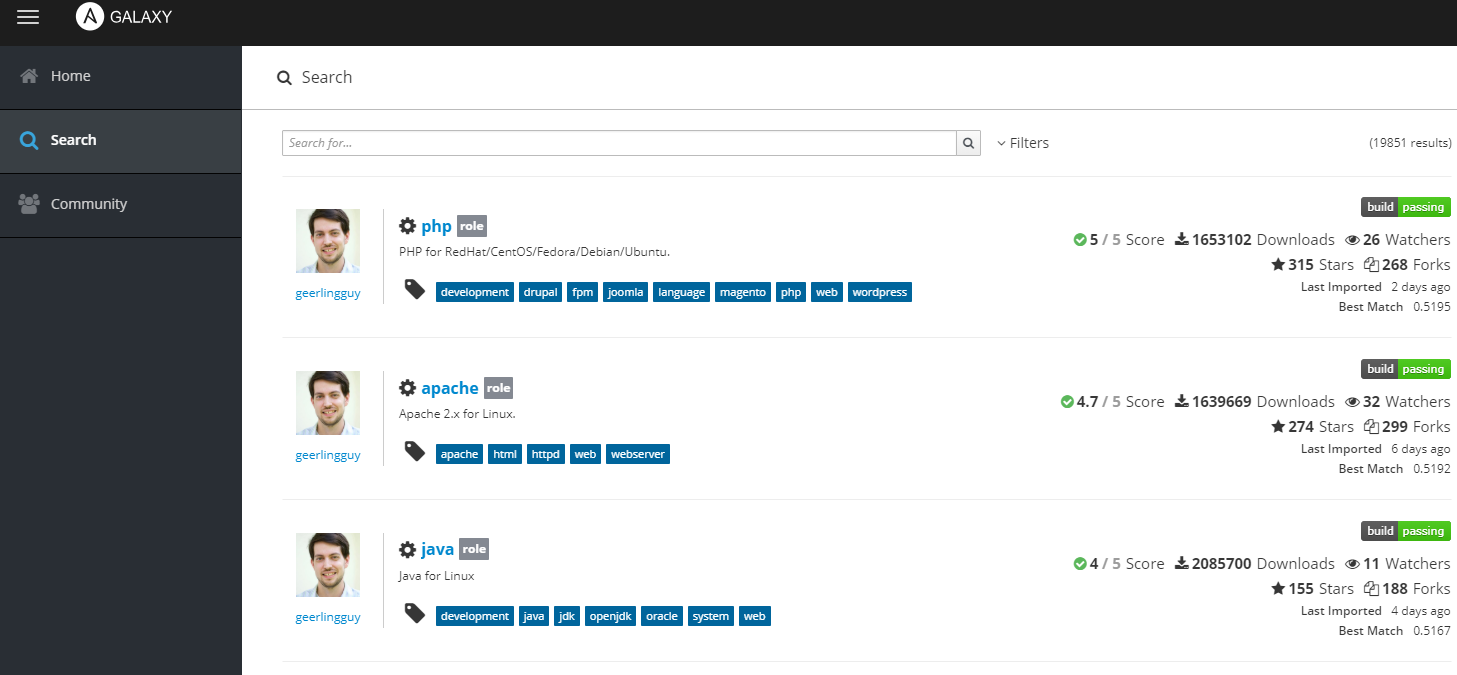
\includegraphics[width=0.9\textwidth]{img/agalaxy.png}}
	\caption{Ansible Galaxy site met lijst van roles.}
	\label{fig:agalaxy}
\end{figure}


\subsection{Omgevingen}
Ansible is even makkelijk te deployen in publieke of private cloud omgevingen, als in een lokale omgeving. Voor publieke of private cloud providers kan er gekozen worden voor: Amazon Web Services, Microsoft Azure, Rackspace,... Maar er kan ook op lokale infrastructuren gewerkt worden door middel van virtuele machines. Tools die hiervoor worden gebruikt zijn: VirtualBox, VMWare,...

\section{Cloud-Init}
\label{ch:cloud-init}
Net als Ansible is cloud-init ook een type van configuration manager en deployment tool. Op de site van cloud-init \autocite{cloudsite} wordt het ontstaan beschreven. Het is ontwikkeld en uitgebracht als gratis software met de open source licentie en ook de Apache Version 2.0 licentie. De makers, Scott Moser en Joshua Harlow, hebben het in python geschreven.

Cloud-init zorgt  voor de customisaties tijdens het opstarten van de cloud of virtuele instanties. Deze service gebeurt heel vroeg in het boot proces. De instantie zoekt naar de \textit{user data} (het cloud-init script) van de gebruiker en voert deze uit. 

Veel van de punten die hier verder worden besproken zijn gevonden in de presentatie van \autocite{cloudred}.

\subsection{Modules}
\label{ch:cloudmodules}
Cloud-init heeft 6 hoofdpijlers waar het modules voor gebruikt, namelijk: schijf configuratie, commando's uitvoeren, gebruikers en groepen creëren, beheren van packages, content bestanden schrijven en bootstrappen van Chef en/of Puppet. Er zijn nog andere modules maar dit zijn de 6 hoofdpijlers van cloud-init en daarbij de meeste gebruikte modules. Er kunnen ook zelf modules toevoegd worden door deze in Python te schrijven. Met behulp van de documentatie van \autocite{clouddocs} wordt er per pijler uitleg gegeven.

\subsubsection{Schijf configuratie}
Er is een module die wordt gebruikt voor de schijf configuratie, namelijk \textbf{Disk Setup}. Via deze module kunnen er simpele partities en bestandsystemen worden geconfigureerd. Via de \textit{device\_aliases} richtlijnen kunnen er aliassen worden gemaakt voor de block devices. Zodat er makkelijker naar deze kan worden verwezen. Via de \textit{disk\_setup} richtlijn wordt de partitie configuratie gedaan. De \textit{table\_type} richtlijn wordt gebruikt om de partitie tabel mee te gegeven. Ten laatste is er ook de \textit{fs\_setup} richtlijn deze wordt gebruikt om de systeembestand configuratie te doen.

\subsubsection{Commando's uitvoeren}
Voor het uitvoeren van commando's zijn er 2 modules: \textbf{Runcmd} en \textbf{Bootcmd}. Beide bevatten maar een richtlijn namelijk \textit{runcmd} en \textit{bootcmd}. 

Bij \textit{runcmd} worden de commando's die worden meegegeven elke keer uitgevoerd als het script wordt gedraaid. 

Bij \textit{bootcmd} enkel alleen als de instantie wordt opgestart. Ook worden de commando's bij \textit{bootcmd} veel vroeger in het bootproces uitgevoerd.

\subsubsection{Gebruikers en groepen}
Ook voor Gebruikers en groepen is er slechts één module: \textbf{Users and Groups}. 

Groepen kunnen worden toegevoegd door deze aan de richtlijn \textit{groups} toe te voegen samen eventuele configuratie per groep. 

Gebruikers kunnen dan weer toegevoegd worden door deze aan de richtlijn \textit{users} toe te voegen. Ook bij de gebruikers kan er nog extra configuratie gedaan worden per gebruiker.

\newpage
\subsubsection{Packages}
Voor het beheren en configureren van packages zijn er verschillende modules: \textbf{Apt Configure}, \textbf{Apt Pipelining}, \textbf{Package Update Upgrade Install}, \textbf{Snap}, \textbf{Snappy} en \textbf{Yum Add Repo}. Er kunnen packages geïnstalleerd en geconfigureerd worden via Yum en Apt. Meestal ondersteunt een besturingssysteem Yum of Apt. Voor de installatie van een package moeten deze geplaatst worden bij de richtlijn \textit{packages}. Cloud-init weet zelf of het met yum of apt wordt gedaan. De configuratie en het toevoegen van package repo's gebeurt via Apt Configure, Apt Pipelinig en Yum Add Repo. Ook ondersteunt cloud-init de installatie van snap packages. Dit zijn gecontaineriseerde packages. Via Snappy kan deze geconfigureerd worden.

\subsubsection{Content bestanden}
Voor het aanmaken van bestanden is er de module \textbf{Write Files}. In de richtlijn \textit{write\_files} word de gecodeerde inhoud van het bestand gezet met het pad.

\subsubsection{Chef - Puppet}
Ook zijn er 2 modules die Chef en Puppet installeren, configureren en starten. Deze modules zijn logischer wijs \textbf{Chef} en \textbf{Puppet}. Voor Puppet wordt de richtlijn \textit{puppet} meegegeven. Daaronder worden alle configuraties geplaatst. Chef werkt op dezelfde manier.

\subsection{User Data - Cloud config}
Net zoals Ansible zijn playbook heeft, heeft cloud-init zijn user data. Ook heeft cloud-init de meta-data, maar deze wordt meegegeven door het cloud platform zelf. Dit zijn bijvoorbeeld de server naam en het server id. De 2 bekendste methodes om user data mee te geven zijn User-Data Script en Cloud Config Data. 

\subsubsection{User-Data Script}
Het User-Data script een Linux script dat de server overloopt voor dat hij opstart. Het moet altijd beginnen met \textit{!\#} of \textit{Content-Type: text/x-shellscript}. Als er echt wordt gebruikt gemaakt van cloud-init wordt deze methode niet gebruikt. De modules kun je via zo een script bijvoorbeeld niet aanroepen. Dit is eerder voor gebruikers die al een script hebben. In plaats van dit om te zetten naar Cloud Config Data, kunnen ze dat dan script gebruiken. Figuur \ref{fig:udatascript} is een voorbeeld van een user-data script.
\begin{figure}[!htb]
	\center{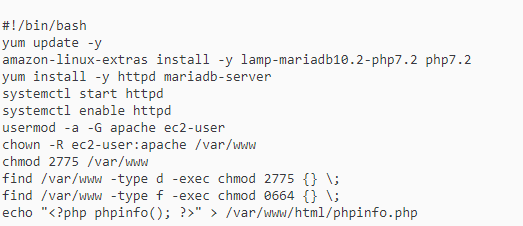
\includegraphics[width=0.9\textwidth]{img/userdatascript.png}}
	\caption{Voorbeeld User-Data Script.}
	\label{fig:udatascript}
\end{figure}
\newpage
\subsubsection{Cloud Config Data}
De populairste methode is Cloud Config Data. Dit is een yaml bestand met de configuratie van de server in. Een Cloud Config bestand begint altijd met \textit{\#cloud-config}. In het bestand worden de modules opgelijst die worden gebruikt en daaronder dan hun configuraties. Dit bestand is veel overzichtelijker dan een script om later aan te passen of om te beheren. Ook heeft het wat gelijkenissen met het playbook van Ansible, doordat dit beide yaml bestanden zijn. Figuur \ref{fig:cloudconfig} is een voorbeeld een cloudconfig bestand.
\begin{figure}[!htb]
	\center{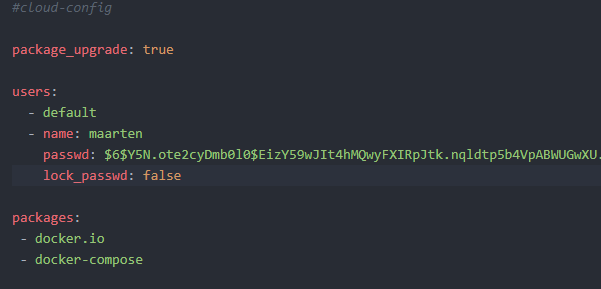
\includegraphics[width=0.9\textwidth]{img/cloudconfig.png}}
	\caption{Voorbeeld Cloud Config Data.}
	\label{fig:cloudconfig}
\end{figure}

\newpage
\subsection{Omgevingen}
De naam van het programma zegt al genoeg. Cloud-init is een service gemaakt voor cloud instanties en cloud platformen. Bij cloud platformen heb je de optie om user data toe te voegen aan de server(s) die je opstart. Meestal is dat een tekst vak waar je data kan invoeren. Dit kan een User-Data script zijn of een Cloud Config bestand. Voorbeelden van cloud platformen zijn: RackSpace, Amazon Web Services, Hetzner en IBM. 

Het is mogelijk om er lokaal mee te werken. Op de server in kwestie moet de package cloud-init worden geïnstalleerd en dan via die package de user data uitvoeren. Je kan deze package installeren en uitvoeren op je host systeem, maar ook in een virtuele omgeving. Programma's om hiervoor te gebruiken zijn: Hyper-V, VMWare en VirtualBox.

\subsection{Systemen}
Volgens de site van cloud-init \autocite{cloudsite} is het oorspronkelijk gemaakt voor Ubuntu systemen. Maar door het succes van de software is het nu beschikbaar op bijna elk Linux systeem: Fedora, Redhat, CentOS,..


